\ifx\wholebook\relax\else
\input{../Common.tex}
\input{../macroes.tex}
\begin{document}
\fi

\chapter*{About this Book}

\begin{quote}\textit{Knowledge is only one part of understanding. Genuine understanding comes from hands on experience. S. Papert}
\end{quote}

\section*{Goals and Audience}
The goal of this book is to explain elementary programming concepts (such as loops, abstractions, composition, and conditionals) to novices of all ages. I believe that learning by experimenting and solving problems is central to human knowledge acquisition. Therefore I present the concepts through simple problems such as drawing golden rectangles or simulating animal behaviors. 

My ultimate goal is to teach you object-oriented programming because it provides an excellent metaphor for teaching programming. However, teaching object-oriented programming requires some notions of programming and abstraction. Therefore, I wrote this book to present these basic programming concepts with the special perspective that this book is the first of a series of two books. The current book is completely self-contained and does not require you to read the next one. The second book introduces a another small environment. It focuses on intermediate-level topics such as finding a path through a  maze or drawing fractals. It also acts as a companion book for people who want to know more, who want to adapt the current environment to their own needs and  it  introduces object-oriented programming. 

The ideal reader I have in mind is a person that wants to have fun programming. This person may be a teenager or an adult, a teacher in high-school, or somebody willing to teach programming to kids in any organization. This person does not have to be fluent in programming in \emph{any} language. 

The material of this book has been originally developed for my wife, who is a physics and mathematics teacher in a french school (where the students  are between 11 and 15 years old). In late 1998, my wife had to teach computer sciences and we got frustrated by the lack of appropriate material. We were dreaming about a way to teach a process of facing problems and finding solutions. My wife started to teach HTML, Word and other topics and she was absolutely not satisfied, since really few approaches  promoted a scientific attitude.  

In addition I was aware of the work on Logo and liked the idea of experimentation as a basis for learning. I was aware that Smalltalk was influenced by the ideas of Papert and Logo, and that it originated from research on teaching programming to kids. Moreover Smalltalk has a simple syntax that mimics natural language. At that time \sq arrived at a mature state and books started to become available in late 1999. So I started and wrote the present book. 

The environments I use in this book and its companion book are fully working, and went through several iterations of improvements based on the feedback I got from teachers. 
A guiding rule in our work has been to modify the \sq environment as little as possible, as our goal is that readers will be able to extend these ideas and develop others later on. 


\section*{Shape and Vocabulary} 

The chapters of this book are relatively small. The idea is that each chapter can be turned into a one or two hours lab session. I do not propose directly usable out of the box teaching material that can be given to kids but each chapter has all the material for that. 

In this book, even if I do not present object-oriented programming, I use its vocabulary \ie we create objects from classes and send them messages. Object behavior is defined by methods. I made this choice because the metaphor offered by object-oriented programming is natural and kids understand well the notion of objects. 

The people used to Logo may wonder why our turtles do not have a pen up and pen down methods but instead go and jump where the go lets a trace while the jump move a turtle forward without letting a trace. As I already mentioned it, the underlying idea behind this book is to create a path to teach object-oriented programming and promote the encapsulation of data, therefore my design is more adapted to than the traditional pen down and pen up design.  I should say that this excellent analysis was made by Didier Besset my early co-author that dropped off the project. 

\section*{Book Structure}
The book is structured in the following five parts. I added an example of the visual effects obtained by the programs used as example in the parts. 

\begin{description}
\item{\bold{Getting Started.}}
The first part shows how to get started with the environment. It presents how to launch \sq and present the robot and their behavior. It shows a first simple program that draws some lines.
\begin{center}

\includegraphics[width=5cm]{ChTurntitlePicture}
\end{center}
\item{\bold{Elementary Programming Concepts.}}
This part introduces the first programming concepts such as loops, variables... It presents how the messages sent to a robot are resolved. 
\begin{center}
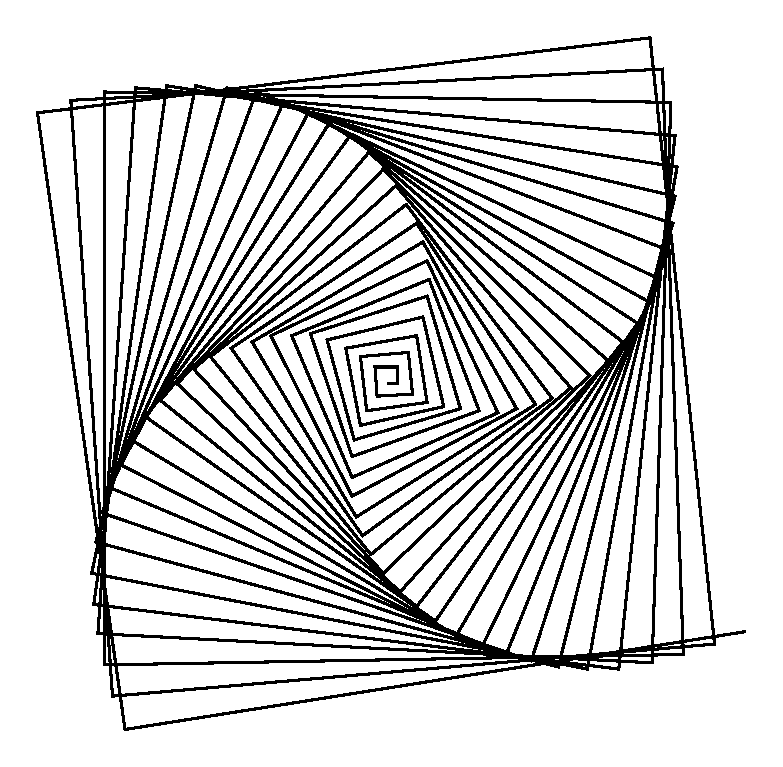
\includegraphics[width=4cm]{varLoopsTitle}
\end{center}
\item{\bold{Bringing Abstraction into Play.}} This part introduces the necessity of having abstraction \ie method or procedures that can be reused by different programs. The most difficult concept introduced is the idea of composing new methods from existing ones to solve more complex problems. Several non trivial experiments are proposed such as drawing golden rectangles. It introduces also techniques and tools to debug programs. 
\begin{center}
\includegraphics[width=5cm]{nborsteps}
\end{center}
\item{\bold{Conditionals.}} This part introduces the notion of conditional, conditional loops and booleans expressions that are central to programming. This part also introduces the notion of references in a 2D space and some other robot behavior. Then it presents how we can use a robot to simulate the behavior of simple animals. 
\begin{center}
\includegraphics[width=3cm]{followBorder2}\includegraphics[width=3cm]{oppositeBorderOfBox}
\end{center}

\item{\bold{Other Programming Environments.}}
This part presents two other environments available in \sq to have fun programming:  The eToy graphical scripting system is presented as well as Alice the 3D-authoring environment.
\end{description}


\section*{Why Squeak and Smalltalk?}

You may wonder why I use Smalltalk and why you would have a learn it in 2004 while a 
lot of other languages exist. I use Smalltalk and Squeak because:

\begin{itemize}
\item Smalltalk is a powerful language. We can build extremely complex systems and still the language is simple and uniform. 

\item Smalltalk was designed to be a language to teach programming. It was influenced by Logo and Lisp, and Smalltalk influenced heavily languages such as Java or C\# but these languages are overly complex and lost the beauty of Smalltalk its simple model. 

\item Smalltalk is dynamically typed and this makes transparent a lot of concerns related to types and types coercion that are tedious to explain for a really limited interest.

\item With Smalltalk you learn the key essential concepts that after you can find in all the other languages. With Smalltalk I can focus on explaining you the important concepts without having to deal with ugly aspects of certain languages. 


\item Squeak is a powerful multimedia environment, so after reading my books you will be able to build your own program in a really rich context. 

\item Squeak is free and runs on all the main platforms of today and can be ported to the ones of the future easily. 

\item Squeak is used in school in Spain on 80 000 computers. 
\end{itemize}

For all these reasons I choose Squeak. 



\section*{Thanks}
I would like to thanks all the people that read this book and gave feedback. I know this was not easy to read parts of a book on progress. I do not want to list you all here as I'm sure that I will forget people. However I want to thank the person who read the book entirely: Orla Greevy, Ian Prince and Daniel Knierim. I just want to thank you for your feedback and support. I have a particular thought to Daniel Villain who read the draft of the french version and died too early. 

I want to thank the Squeak community for the help it provided me during the development of the environments used in this book, and for developing Squeak this amazing environment. I have a special thank for all the developers that made Smalltalk escaping clouds of dream and becoming reality. I would like to thank all the Smalltalkers that make this language and community so exciting. Continue to make your dreams come true. 

Writing this book was a long and difficult process because teaching novices is difficult. Moreover I'm not an easy person to live with and a researcher that is excited by too much topics.  I want to thanks Didier Besset for the discussions we got even if at the end we were not synchronized.

I also  want to thank my wife Florence, and Quentin, and Thibaut  these two small boys that are running and shouting around my desk when I would like to be concentrated to accept a husband and father that is not always present, enthusiast and accessible. 

\ifx\wholebook\relax\else\end{document}\fi

